\documentclass[12pt,a4paper]{article}

% --- PAKETE FÜR DEUTSCHE SPRACHE & SCHRIFTART ---
\usepackage[T1]{fontenc}
\usepackage[ngerman]{babel}
\usepackage{lmodern}
\usepackage{graphicx}

% --- CSQUOTES (Vom Biblatex-Paket empfohlen) ---
\usepackage{csquotes}

% --- MATHE, ENUMERATE, FLOAT & LAYOUT ---
\usepackage{amsmath,amssymb}
\usepackage{geometry}
\geometry{a4paper, margin=2.5cm}
\usepackage{parskip}
\usepackage{enumitem}
\usepackage{float}

% --- TCOLORBOX FÜR HIGHLIGHT- & AUFGABENBOXEN ---
\usepackage[most]{tcolorbox}

\newtcolorbox{taskbox}[1][]{
    colback=blue!5!white,
    colframe=blue!60!black,
    fonttitle=\bfseries,
    title={#1},
    arc=2mm,
    boxrule=0.8pt,
    left=4mm, right=4mm, top=3mm, bottom=3mm
}

\newtcolorbox{solutionbox}[1][Lösung]{
    colback=green!5!white,
    colframe=green!50!black,
    fonttitle=\bfseries,
    title={#1},
    arc=2mm,
    boxrule=0.8pt,
    left=4mm, right=4mm, top=3mm, bottom=3mm
}

\newtcolorbox{emailbox}[1][]{
    colback=red!4!white,
    colframe=red!65!black,
    fonttitle=\bfseries,
    title={#1},
    arc=1.5mm,
    boxrule=0.8pt,
    left=4mm, right=4mm, top=3mm, bottom=3mm
}

% --- FARBEN & VERLINKUNGEN ---
\usepackage{xcolor}
\usepackage[colorlinks=true, linkcolor=blue!60!black, urlcolor=blue!60!black, citecolor=blue!60!black]{hyperref}

% --- CLEVEREF (MUSS NACH HYPERREF GELADEN WERDEN) ---
\usepackage[ngerman]{cleveref}
\crefname{figure}{Abbildung}{Abbildungen}
\Crefname{figure}{Abbildung}{Abbildungen}
\crefname{table}{Tabelle}{Tabellen}
\Crefname{table}{Tabelle}{Tabellen}
\crefname{section}{Abschnitt}{Abschnitte}
\Crefname{section}{Abschnitt}{Abschnitte}

% --- LITERATURVERZEICHNIS MIT BIBLATEX & BIBER ---
\sloppy
\usepackage[backend=biber, style=numeric]{biblatex}
\addbibresource{literatur.bib}

% --- GLOSSAR & ABKÜRZUNGSVERZEICHNIS ---
\usepackage[toc, acronym, nonumberlist]{glossaries}
\makeglossaries

% Custom Glossar-Style für optisch ansprechende Formatierung
\newglossarystyle{mycleanstyle}{%
  \setglossarystyle{long}%
  \renewenvironment{theglossary}%
     {\begin{longtable}{@{}p{5.8cm}@{\hspace{0.6cm}}p{9.6cm}@{}}}%
     {\end{longtable}}%
  \renewcommand*{\glossentry}[2]{%
    \textbf{\glsentryname{##1}} & \glsentrydesc{##1}\\[0.9em]%
  }%
  \renewcommand*{\glsgroupskip}{}%
}
\setglossarystyle{mycleanstyle}

% Inkludieren der separaten Abkürzungs- und Glossardateien
% --- ABKÜRZUNGEN (AKRONYME) ---

\newacronym{mfa}{MFA}{Multi-Faktor-Authentisierung}
\newacronym{nist}{NIST}{National Institute of Standards and Technology}
\newacronym{bsi}{BSI}{Bundesamt für Sicherheit in der Informationstechnik}
\newacronym{smtp}{SMTP}{Simple Mail Transfer Protocol}
\newacronym{url}{URL}{Uniform Resource Locator}
\newacronym{it}{IT}{Informationstechnik}
\newacronym{ki}{KI}{Künstliche Intelligenz}

% --- GLOSSAREINTRÄGE ---

\newglossaryentry{Multi-Faktor-Authentisierung}{
    name={Multi-Faktor-Authentisierung},
    description={Ein Sicherheitsverfahren, bei dem mehrere unabhängige Faktoren zur Authentifizierung kombiniert werden.}
}

\newglossaryentry{passwort}{
    name={Passwort},
    description={Eine geheime Zeichenkette, die zur Authentisierung dient.}
}

\newglossaryentry{entropie}{
    name={Entropie},
    description={Mass für die mathematische Stärke und die Unsicherheit des Erzeugungsverfahrens bei der Generierung eines \gls{passwort}s in \gls{bit}. Die Berechnungsformel setzt eine rein zufällige und unabhängige Auswahl voraus; bei manuell gewählten \glslink{passwort}{Passwörtern} überschätzt sie die tatsächliche Stärke. Entropie aus dem \gls{suchraum} $N$:
    \[
    E = \log_2(N)
    \]
    Für Zeichen-Passwörter gilt $N = R^L$ (Zeichenvorrat $R$, Länge $L$), für Wort-Passphrasen gilt $N = W^L$ (Wörterbuchgrösse $W$, Länge $L$ in Wörtern).}
}

\newglossaryentry{bruteforce}{
    name={Brute-Force-Angriff},
    description={Ein automatisierter Angriff, bei dem Programme alle möglichen Zeichenkombinationen systematisch \mbox{durchprobieren}.}
}

\newglossaryentry{dictionaryattack}{
    name={Dictionary Attack (Wörterbuchangriff)},
    description={Ein gezielter Angriff, bei dem Listen mit \mbox{gebräuchlichen} Wörtern, Namen und bekannten Passwörtern systematisch getestet werden.}
}

\newglossaryentry{datenleck}{
    name={Datenleck},
    description={Ein Vorfall, bei dem vertrauliche Daten unabsichtlich oder absichtlich veröffentlicht oder gestohlen werden.}
}

\newglossaryentry{passwortmanager}{
    name={Passwort-Manager},
    description={Software zur sicheren Verwaltung und Generierung von Passwörtern.}
}

\newglossaryentry{passphrase}{
    name={Passphrase},
    description={Eine längere Zeichenkette, oft bestehend aus mehreren zufälligen Wörtern, die als Passwort verwendet wird.}
}

\newglossaryentry{phishing}{
    name={Phishing},
    description={Eine Form des Social Engineering, bei der Angreifer versuchen, über gefälschte E-Mails, Nachrichten oder Webseiten an vertrauliche Daten zu gelangen.}
}

\newglossaryentry{socialengineering}{
    name={Social Engineering},
    description={Die Manipulation von Personen durch psychologische Tricks, um an vertrauliche Informationen zu gelangen.}
}

\newglossaryentry{spearphishing}{
    name={Spear-Phishing},
    description={Ein gezielter Phishing-Angriff, der auf eine spezifische Person oder bestimmte Mitarbeiter zugeschnitten ist.}
}

\newglossaryentry{quishing}{
    name={Quishing},
    description={Eine Phishing-Methode, bei der manipulierte QR-Codes eingesetzt werden, um Opfer auf gefälschte Webseiten zu leiten.}
}

\newglossaryentry{vishing}{
    name={Vishing},
    description={Eine Phishing-Methode, bei der Angreifer telefonisch versuchen, vertrauliche Informationen zu erlangen.}
}

\newglossaryentry{klassischesphishing}{
    name={Klassisches Phishing},
    description={Eine Phishing-Methode, bei der Angreifer E-Mails oder Nachrichten an eine breite Masse von Personen senden, um an vertrauliche Informationen zu gelangen.}
}

\newglossaryentry{smishing}{
    name={Smishing},
    description={Eine Phishing-Methode, bei der Angreifer über SMS versuchen, vertrauliche Informationen zu erlangen.}
}

\newglossaryentry{typosquatting}{
    name={Typosquatting},
    description={Eine Technik, bei der Angreifer Domains registrieren, die ähnlich zu bekannten Webseiten sind, um Nutzer durch Tippfehler auf gefälschte Seiten zu locken.}
}

\newglossaryentry{pin}{
    name={PIN},
    description={Eine persönliche Identifikationsnummer, oft verwendet zur Authentifizierung von Nutzern.}
}

\newglossaryentry{suchraum}{
    name={Suchraum},
    description={Der gesamte mögliche Suchraum für ein \gls{passwort} oder einer \gls{passphrase}, bestehend aus allen möglichen (Zeichen)-Kombinationen.}
}

\newglossaryentry{bit}{
    name={Bit},
    description={Ein Bit ist die kleinste Einheit digitaler Information, die zwei Zustände (0 oder 1 / an oder aus) darstellen kann.}
}

\newglossaryentry{livephishing}{
    name={Live-Phishing},
    description={Beim Live-Phishing schalten Kriminelle eine gefälschte Website dazwischen, um Passwort und Einmalcode (MFA) in Echtzeit abzufangen und sich sofort auf der echten Seite einzuloggen.}
}

\begin{document}

% --- TITELBLATT ---
\begin{titlepage}
    \pagenumbering{gobble}
    \centering
    \vspace*{2cm}
    
    {\Huge \textbf{Skript: Passwortsicherheit \& Phishing} \par}
    \vspace{1.5cm}
    {\Large \textbf{Kantonsschule im Lee} \par}
    \vspace{2cm}
    
    \rule{\linewidth}{0.5mm}
    \vspace{2cm}
    
    {\large \textbf{Thema:} Passwortsicherheit, Phishing, Entropie \& Best Practices \par}
    \vspace{0.5cm}
    {\large \textbf{Fach:} Informatik \par}
    \vspace{0.5cm}
    {\large \textbf{Autor:} Laurin Ott \par}
    
    \vfill
    
    {\large \textbf{Datum:} \today \par}
\end{titlepage}

% --- INHALTSVERZEICHNIS ---
\newpage
\pagenumbering{arabic}
\tableofcontents
\newpage

% --- TEIL 1: PASSWORTSICHERHEIT ---
\section{Passwortsicherheit}
\label{sec:passwortsicherheit}

\subsection{Einleitung}
In fast allen IT-Systemen bilden \glslink{passwort}{Passwörter} die erste Hürde gegen unbefugten Zugriff. In der Praxis zeigt sich jedoch immer wieder, dass schwache, kompromittierte oder mehrfach genutzte \glslink{passwort}{Passwörter} eine der grössten Sicherheitslücken darstellen. Dieses Skript gibt einen Überblick über die mathematischen Grundlagen der \gls{passwort}-Stärke und fasst die aktuellen Empfehlungen zur Absicherung digitaler Identitäten zusammen \cite{nist2025}.

\subsection{Grundlegende Begriffe und Angriffsarten}
In der Authentisierung und \gls{passwort}-Sicherheit spielen verschiedene Konzepte und Bedrohungen eine entscheidende Rolle. Neben dem rein mathematischen \gls{bruteforce} nutzen Angreifer in der Praxis sehr häufig einen \glslink{dictionaryattack}{Wörterbuchangriff}, bei dem gezielt Listen mit geläufigen Wörtern, Namen und bekannten Daten \mbox{durchprobiert} werden. Um diesen \mbox{Methoden} zu entgehen, ist eine hohe \gls{entropie} entscheidend. \\ Zusätzlich erhöht moderne \gls{mfa} (z. B. eine Bestätigung direkt auf dem Smartphone) die Sicherheit deutlich, da ein Passwort allein meist nicht mehr ausreicht.

\subsection{Mathematische Grundlage: Die Passwort-Entropie}
\label{subsec:entropie}
Die Stärke eines \gls{passwort}s beschreibt die \glslink{entropie}{Shannon-Entropie (E)} seines Erzeugungsverfahrens. Sie beschreibt den Grad der Zufälligkeit bei der Erstellung eines Passworts und wird in der Einheit \gls{bit} angegeben. Ein \gls{bit} entspricht dabei einer binären Entscheidung (1/0), die ein Computer benötigt, um den \mbox{möglichen} \gls{suchraum} Schritt für Schritt \\ einzuschränken. Unter der Bedingung, dass alle Zeichen völlig zufällig und unabhängig voneinander gewählt werden (wie bei der Generierung durch einen \gls{passwortmanager}), berechnet sich die \gls{entropie} wie folgt:   
$$N=R^L$$
$$E = \log_2(N) = \log_2(R^L) = L \cdot \log_2(R)$$
Für \gls{passphrase}n gilt die Formel:
$$N = W^L$$
$$E = \log_2(N) = \log_2(W^L) = L \cdot \log_2(W)$$
\begin{itemize}
    \item $N$: Anzahl der möglichen Zeichen Kombinationen für das \gls{passwort} oder Wörter Kombinationen für die \gls{passphrase} (\gls{suchraum}).
    \item $E$: \gls{entropie} in \gls{bit} (Mass für die Stärke des \gls{passwort}s).
    \item $L$: Die Länge des \gls{passwort}s (Anzahl der verwendeten Zeichen) oder die Länge der \gls{passphrase} (Anzahl der verwendeten Wörter).
    \item $R$: Die Grösse des verfügbaren Zeichensatzes (z.\,B. Kleinbuchstaben, \\ Grossbuchstaben, Zahlen, Sonderzeichen).
    \item $W$: Die Anzahl der Wörter in dem Wörterbuch.
\end{itemize}
Wichtig ist, dass diese Formel echte Zufallsauswahl voraus setzt. Selbst gewählte \\ \glslink{passwort}{Passwörter} (wie z. B. Sommer2026!) besitzen eine deutlich geringere \gls{entropie}, da \\ menschliche Eingaben meist vorhersehbaren Mustern folgen und dadurch der tatsächliche \gls{suchraum} für Angreifer stark schrumpft. Das Gleiche gilt für \gls{passphrase}n. \gls{passphrase}n sind mehrere zufällige Wörter, die zu einer langen Wörterkette kombiniert werden.
\subsubsection{Beispielrechnung}
\begin{itemize}
    \item \textbf{8 Zeichen (nur Kleinbuchstaben):} Bei $L = 8$ und einem Zeichensatz von $R = 26$ ergibt sich eine \gls{entropie} von:
    \[
    E_8 = 8 \cdot \log_2(26) \approx 37{,}6 \text{ Bit}
    \]
    \item \textbf{Verdopplung auf 16 Zeichen (gleicher Zeichensatz):} Bei $L = 16$ und $R = 26$ steigt die \gls{entropie} linear mit der Länge auf:
    \[
    E_{16} = 16 \cdot \log_2(26) \approx 75{,}2 \text{ Bit}
    \]
\end{itemize}

In \cref{tab:entropie_vergleich} sind die \gls{entropie}-Werte für verschiedene \gls{passwort}-Längen und Zeichensätze zusammenfassend dargestellt.

\begin{table}[htbp]
    \centering
    \begin{tabular}{|l|c|c|r|}
        \hline
        \textbf{Zeichensatz ($R$)} & \textbf{Länge ($L$)} & \textbf{Formel} & \textbf{\gls{entropie} ($E$)} \\
        \hline
        Kleinbuchstaben ($R=26$) & 8 & $8 \cdot \log_2(26)$ & $\approx 37{,}6$ Bit \\
        Kleinbuchstaben ($R=26$) & 16 & $16 \cdot \log_2(26)$ & $\approx 75{,}2$ Bit \\
        Alle Zeichen ($R=94$) & 8 & $8 \cdot \log_2(94)$ & $\approx 52{,}4$ Bit \\
        Kleinbuchstaben ($R=26$) & 20 & $20 \cdot \log_2(26)$ & $\approx 94{,}0$ Bit \\
        Alle Buchstaben ($R=52$) & 20 & $20 \cdot \log_2(52)$ & $\approx 114{,}0$ Bit \\
        Alle Buchstaben + Zahlen ($R=62$) & 20 & $20 \cdot \log_2(62)$ & $\approx 119{,}1$ Bit \\
        Alle Zeichen ($R=94$) & 20 & $20 \cdot \log_2(94)$ & $\approx 131{,}1$ Bit \\
        \hline
    \end{tabular}
    \caption{Vergleich der \gls{passwort}-\gls{entropie} für verschiedene Längen und Zeichensätze.}
    \label{tab:entropie_vergleich}
\end{table}

\subsubsection{Fazit der Berechnung}
Weil die Anzahl der möglichen Kombinationen ($N = R^L$) exponentiell mit der Länge ($L$) wächst, erhöht jedes zusätzliche Zeichen die Sicherheit drastisch. Die \gls{entropie} ($E = L \cdot \log_2(R)$) wächst zwar linear mit der Länge und nur logarithmisch mit der Zeichensatzauswahl ($R$). Für die Praxis bedeutet das aber, ein längeres \gls{passwort} bietet um ein Vielfaches mehr Schutz als das krampfhafte Einfügen von Sonderzeichen in ein zu kurzes \gls{passwort}. Zudem schützt eine ausreichende Länge in Kombination mit Zufall effektiv vor \gls{dictionaryattack}s.

\newpage

\subsection{Aktuelle Richtlinien und Best Practices}
Moderne Richtlinien haben sich von alten Regeln verabschiedet. Heute gelten folgende Hauptempfehlungen:
\begin{enumerate}
    \item \textbf{Länge vor Komplexität:} Bevorzugung von \gls{passphrase}n aus mehreren \mbox{zufälligen} Wörtern. Selbst wenn Angreifer raffinierte Wörterbuchangriffe oder Kombinationen ausprobieren, bricht ein System bei langen Passphrasen \mbox{(oft auch ohne erzwungene Sonderzeichen)} ein, weil die schiere Länge den Suchraum unknackbar macht (bei einer \gls{diceware} von 7776 Wörtern wird eine \\ \gls{entropie} von über 80 \gls{bit} ab 7 rein zufällig gewählten Wörtern erreicht). (3.1.1.2 \cite{nist2025})
    \item \textbf{Keine wiederholte Nutzung von \glslink{passwort}{Passwörtern}:} Jedes Konto sollte ein \mbox{einzigartiges} \gls{passwort} besitzen, um die Risiken bei \gls{datenleck}s zu minimieren. (3.1.1.2.4 \cite{nist2025})
    \item \textbf{Vermeidung von \gls{passwort}-Änderungen ohne Anlass:} Regelmässige \mbox{erzwungene} \gls{passwort}-Änderungen erhöhen die Wahrscheinlichkeit, dass Nutzer schwächere \glslink{passwort}{Passwörter} wählen oder diese aufschreiben. Nur bei Verdacht auf Kompromittierung sollte ein \gls{passwort} geändert werden. (3.1.1.2 \cite{nist2025})
    \item \textbf{Einsatz von \gls{passwortmanager}n:} Generierung und Verwaltung einzigartigen \mbox{\glslink{passwort}{Passwörtern}}. (3.1.1.2 \cite{nist2025})
    \item \textbf{Aktivierung von \gls{mfa}:} Einrichtung eines zweiten Faktors (z.\,B. aufs \mbox{Smartphone}). (2.1 und 2.2 \cite{nist2025})
\end{enumerate}

\newpage
% --- TEIL 2: PHISHING ---
\section{Phishing}
\label{sec:phishing}

\subsection{Einleitung}
In der digitalen Welt bilden nicht nur technische Barrieren wie \glslink{passwort}{Passwörter} die \mbox{Abwehrlinie}, sondern vor allem der Mensch selbst. Eines der erfolgreichsten und am \mbox{häufigsten} genutzten Einfallstore für Cyberkriminelle ist \gls{phishing}. Dabei wird gezielt die \mbox{menschliche Psyche} ausgenutzt, um an vertrauliche Daten zu gelangen oder \mbox{Schadsoftware} zu verbreiten.

\subsection{Grundlegende Begriffe und Angriffsarten}
\gls{phishing} gehört zu den klassischen \gls{socialengineering}-Angriffen. Statt komplexe \mbox{technische Systeme} direkt zu hacken, manipulieren Angreifer gezielt Personen:
\begin{itemize}
    \item \textbf{\gls{klassischesphishing}:} Täuschend echte E-Mails, die \mbox{vorgeben}, von \mbox{vertrauenswürdigen} \mbox{Institutionen} \newline (wie Banken, Streaming-Diensten oder Behörden) zu \mbox{stammen}. \cite{cisaphishingpostcard,bacsphishing}
    \item \textbf{\gls{spearphishing}:} Ein gezielter Angriff (\gls{spearphishing}), der auf eine spezifische Person oder bestimmte Mitarbeiter zugeschnitten ist, um Vertrauen zu erwecken. \cite{cisaphishingpostcard,niccsglossary}
    \item \textbf{\gls{vishing} \& \gls{smishing}:} Betrugsversuche über Telefonanrufe (\textit{Voice \rightarrow \gls{vishing}}) oder \mbox{Kurznachrichten} (\textit{SMS \rightarrow \gls{smishing}}). \cite{cisaphishingpostcard,bacsphishing}
    \item \textbf{\gls{quishing}:} Das Platzieren von manipulierten QR-Codes (z. B. auf Plakaten oder Parkuhren), die zu gefälschten Webseiten führen. \cite{bacsphishing}
\end{itemize}

\begin{figure}[H]
    \centering
    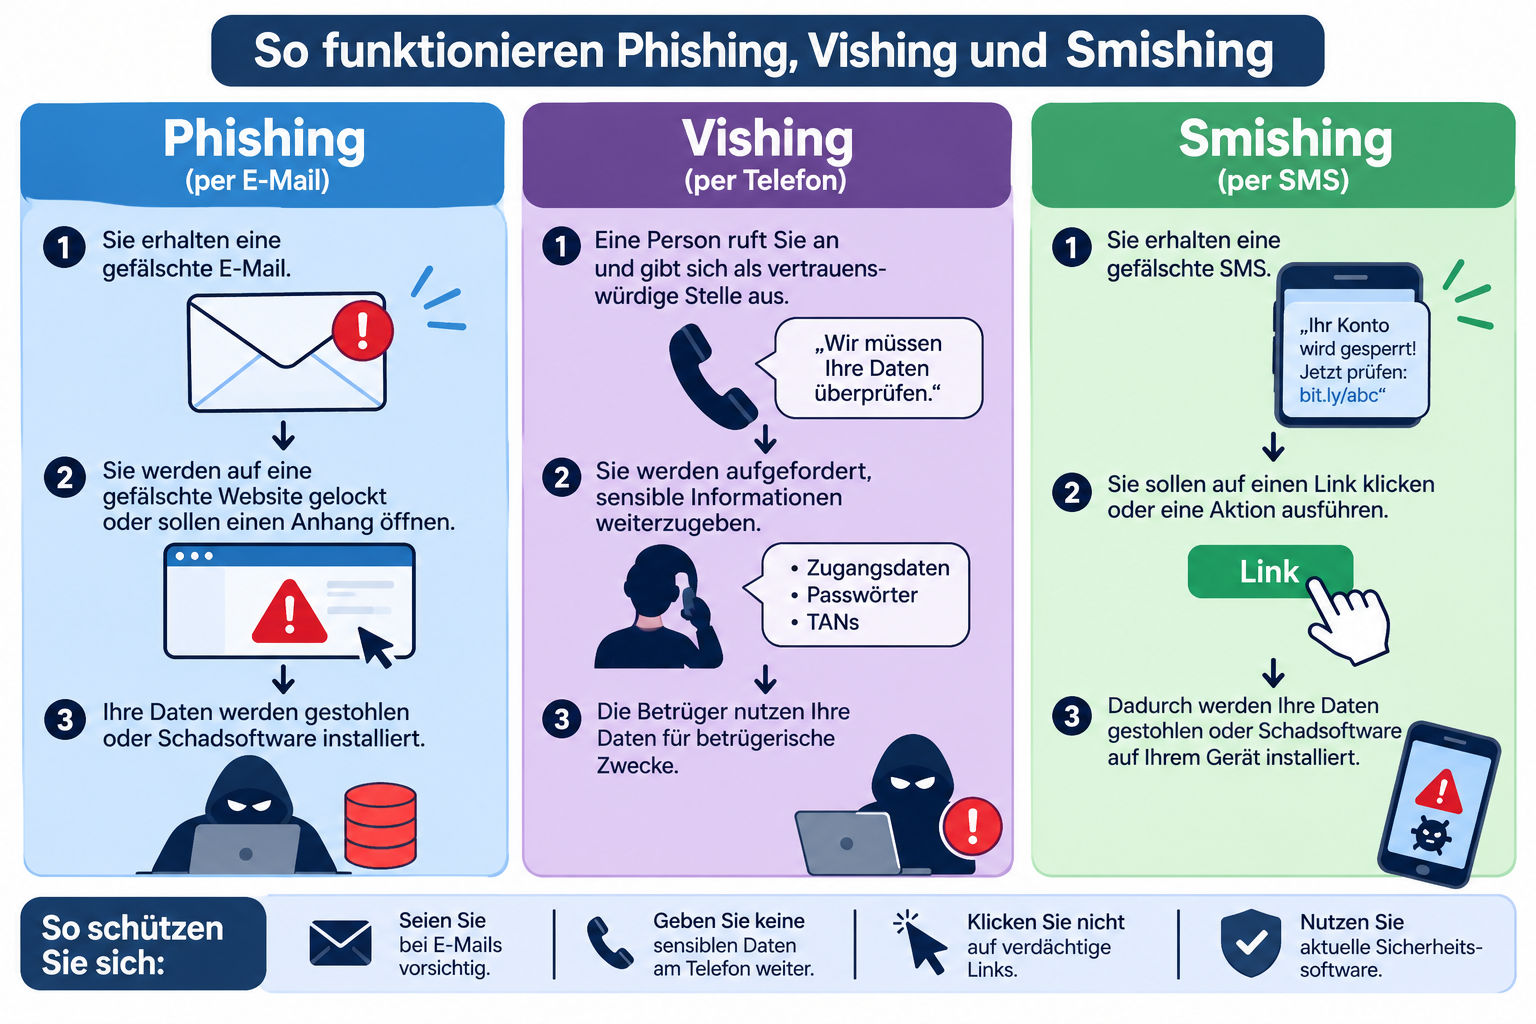
\includegraphics[width=0.9\textwidth]{So_funktionieren_Phishing,_Vishing_und_Smishing.png}
    \caption[Funktionsweise von Phishing, Vishing und Smishing]{Funktionsweise von Phishing, Vishing und Smishing (erstellt mit DALL-E, 31.10.2026).}
    \label{fig:phishing-vishing-smishing}
\end{figure}

\subsection{Psychologische Faktoren und Wirkungsweise}
Im Gegensatz zu mathematischen Angriffen zielt \gls{phishing} auf menschliche Schwachstellen wie Neugier, Hilfsbereitschaft, Gier oder vor allem \textbf{Angst und Zeitdruck} ab. Typische Maschen beinhalten drohende Konsequenzen wie angebliche Kontosperrungen, dringende Rechnungen oder verpasste Gewinne, damit das Opfer unüberlegt handelt. \cite{cisaphishingpostcard,bacsphishing}.

\subsection{Aktuelle Richtlinien und Best Practices}
Um sich vor \gls{phishing}-Angriffen zu schützen, gelten im Rahmen der IT-Sicherheit folgende zentrale Empfehlungen:

\begin{enumerate}
    \item \textbf{Kritische Hürden bewahren:} Niemals unüberlegt auf Links klicken oder \mbox{Anhänge} von unbekannten Absendern öffnen. \cite{cisaphishingpostcard}\cite{bacsphishing}
    \item \textbf{Absender und URLs genau prüfen:} Auf Unstimmigkeiten in E-Mail-Adressen (z. B. Buchstabendreher in Domains (\gls{typosquatting})) achten. \cite{cisaphishingpostcard}\cite{bacsphishing}
    \item \textbf{\gls{mfa} nutzen (und ihre Grenzen bei \gls{livephishing} kennen):} \gls{mfa} erschwert Kontoübernahmen massiv, da beim klassischen Phishing ein abgefangenes \gls{passwort} ohne den zweiten Faktor nutzlos ist. Gegen gezieltes \textbf{\gls{livephishing}} (Adversary-in-the-Middle) bietet Standard-\gls{mfa} jedoch keinen zuverlässigen Schutz. Lockt ein Angreifer das Opfer auf eine gefälschte Login-Seite, werden dort nicht nur das Passwort, sondern auch Einmalcodes (per SMS oder Authenticator-App) abgegriffen und direkt für den Zugriff auf das echte Konto missbraucht. Auch App-basierte Push-Benachrichtigungen lassen sich umgehen, indem Angreifer durch eigene Login-Versuche Bestätigungsanfragen beim Opfer auslösen und dieses so zur Freigabe verleiten. Einen zuverlässigen Schutz gegen solche Phishing-Angriffe bieten daher nur phishing-resistente Verfahren wie \textbf{FIDO2/WebAuthn-Sicherheitsschlüssel oder plattformintegrierte Authentifikatoren (Passkeys)}, da sie auch gegen gefälschte Login-Seiten und abgefangene Eingaben immun sind. \cite{cisaphishingpostcard} \cite{cisamfa}
    \item \textbf{Keine sensiblen Daten preisgeben:} Seriöse Institutionen fragen niemals per E-Mail, SMS oder Telefon nach \glslink{passwort}{Passwörtern} oder \gls{pin}s. \cite{bacsphishing}
    \item \textbf{Dringlichkeit und Druckmittel hinterfragen:} E-Mails, die mit \mbox{unbegründeten} Drohungen (z.~B. sofortige Kontosperrung) oder kurzen Fristen Panik erzeugen \mbox{wollen}, kritisch prüfen. \cite{cisaphishingpostcard}
    \item \textbf{Sprache und Anrede analysieren:} Unpersönliche Anreden (z.~B. „Sehr \mbox{geehrter} Kunde“) sowie grammatikalische Fehler, Rechtschreibfehler, fehlende Umlaute oder auffällige Formulierungen bleiben wichtige Warnsignale für Phishing-Mails. Durch den Einsatz moderner KI-Tools sind Angreifer jedoch zunehmend in der Lage, sprachlich einwandfreie Nachrichten zu erstellen. Daher gilt,dass das Fehlen von Sprachfehlern kein Garantiebeweis für die Echtheit einer Nachricht ist. \cite{cisaphishingpostcard}
    \item \textbf{Direktzugriffe bevorzugen:} Webseiten und Portale stets manuell über die \mbox{Eingabe} der bekannten Adresse im Browser aufrufen, anstatt Links aus E-Mails zu folgen. \cite{cisaphishingpostcard}\cite{bacsphishing}
\end{enumerate}

\newpage
% --- TEIL 3: ÜBUNGSAUFGABEN ---
\section{Übungsaufgaben}
\label{sec:aufgaben}

Dieser Abschnitt enthält Vertiefungs- und Übungsaufgaben zu den Themen aus \mbox{\cref{sec:passwortsicherheit}} und \mbox{\cref{sec:phishing}}.

\subsection{Aufgabenblatt 1: Passwortsicherheit}
\label{subsec:aufgaben_passwort}

\subsubsection{Teil 1: Begriffsdefinitionen \& Grundlagen}

\begin{taskbox}[{Aufgabe 1: Begriffsdefinitionen}]
Erklären Sie kurz in Ihren eigenen Worten den Unterschied zwischen einem \newline Brute-Force-Angriff und einem Dictionary Attack (Wörterbuchangriff).
\end{taskbox}

\begin{solutionbox}[Musterlösung Aufgabe 1]
\begin{itemize}
    \item \textbf{Brute-Force-Angriff:} Ein automatisierter Angriff, bei dem Programme \mbox{systematisch} alle möglichen Zeichenkombinationen durchprobieren.
    \item \textbf{Dictionary Attack (Wörterbuchangriff):} Ein gezielter Angriff, bei dem Listen mit gebräuchlichen Wörtern, Namen und bekannten \glslink{passwort}{Passwörtern} \mbox{systematisch} getestet werden.
\end{itemize}
\end{solutionbox}

\begin{taskbox}[{Aufgabe 2: MFA}]
Was bedeutet die Abkürzung \gls{mfa} und wie schützt sie einen Account, selbst wenn ein Angreifer das \gls{passwort} herausgefunden hat?
\end{taskbox}

\begin{solutionbox}[Musterlösung Aufgabe 2]
\textbf{MFA} steht für \textbf{Multi-Faktor-Authentisierung}. Sie schützt einen Account, indem neben dem \gls{passwort} ein zweiter Faktor (z.\,B. eine Bestätigung auf dem Smartphone) erforderlich ist. Selbst wenn ein Angreifer das \gls{passwort} erlangt hat, wird der Zugriff mit diesem zweiten Faktor erschwert.
\end{solutionbox}

\newpage
\subsubsection{Teil 2: Mathematische Berechnungen (Entropie)}

Verwenden Sie diese Formeln zur Berechnung der \gls{entropie} aus \cref{subsec:entropie} \newline(sehen Sie auch \cref{tab:entropie_vergleich}).
Für \glslink{passwort}{Passwörter} gilt:
\[
E = L \cdot \log_2(R)
\]
Für \gls{passphrase}n gilt:
\[
E = L \cdot \log_2(W)
\]

\begin{taskbox}[{Aufgabe 3: Einfluss des Zeichensatzes ($R$)}]
Gegeben ist ein \gls{passwort} der Länge $L = 10$.
\begin{enumerate}[label=\alph*)]
    \item Berechnen Sie die \gls{entropie} $E$, wenn nur Kleinbuchstaben verwendet werden \newline($R = 26$).
    \item Berechnen Sie die \gls{entropie} $E$, wenn Klein-, Grossbuchstaben, Zahlen und Sonderzeichen verwendet werden ($R = 94$).
\end{enumerate}
\end{taskbox}

\begin{solutionbox}[Musterlösung Aufgabe 3]
\begin{enumerate}[label=\alph*)]
    \item $E = 10 \cdot \log_2(26) \approx 10 \cdot 4{,}7004 = 47{,}0 \text{ Bit}$
    \item $E = 10 \cdot \log_2(94) \approx 10 \cdot 6{,}5546 = 65{,}5 \text{ Bit}$
\end{enumerate}
\end{solutionbox}

\begin{taskbox}[{Aufgabe 4: Einfluss der Länge ($L$) bei \gls{passphrase}n}]
Gegeben ist eine \gls{passphrase} mit der Wörterlistengrösse $W = 7776$.
\begin{enumerate}[label=\alph*)]
    \item Berechnen Sie die \gls{entropie} $E$, für ein Wort ($L = 1$).
    \item Berechnen Sie die \gls{entropie} $E$, wenn nur 5 Wörter verwendet werden \newline($L = 5$).
    \item Berechnen Sie die \gls{entropie} $E$, wenn 7 Wörter verwendet werden ($L = 7$).
\end{enumerate}
\end{taskbox}

\begin{solutionbox}[Musterlösung Aufgabe 4]
\begin{enumerate}[label=\alph*)]
    \item $E = 1 \cdot \log_2(7776) \approx 1 \cdot 12{,}93 = 12{,}93 \text{ Bit}$
    \item $E = 5 \cdot \log_2(7776) \approx 5 \cdot 12{,}93 = 64{,}65 \text{ Bit}$
    \item $E = 7 \cdot \log_2(7776) \approx 7 \cdot 12{,}93 = 90{,}51 \text{ Bit}$
\end{enumerate}
\end{solutionbox}

\begin{taskbox}[{Aufgabe 5: Länge vs. Komplexität}]
Betrachten Sie die folgenden beiden \glslink{passwort}{Passwörter}:
\begin{itemize}
    \item \textbf{Szenario A:} Ein komplexes \gls{passwort} mit 8 Zeichen ($L = 8$), \newline das \mbox{Kleinbuchstaben}, \mbox{Grossbuchstaben}, \mbox{Zahlen} und \mbox{Sonderzeichen} nutzt \newline($R = 94$).
    \item \textbf{Szenario B:} Ein zufälliges \gls{passwort} mit 20 Zeichen ($L = 20$), das nur aus Kleinbuchstaben besteht ($R = 26$).
\end{itemize}
\textbf{Aufgabe:} Berechnen Sie für beide Szenarien die \gls{entropie} $E$. Welches \gls{passwort} bietet eine höhere \gls{entropie} und warum entspricht dies der Regel „Länge vor \mbox{Komplexität}“?
\end{taskbox}

\begin{solutionbox}[Musterlösung Aufgabe 5]
\begin{itemize}
    \item \textbf{Szenario A ($L=8, R=94$):} $E_A = 8 \cdot \log_2(94) \approx 52{,}4 \text{ Bit}$
    \item \textbf{Szenario B ($L=20, R=26$):} $E_B = 20 \cdot \log_2(26) \approx 94{,}0 \text{ Bit}$
\end{itemize}
\textbf{Auswertung \& Begründung:} Szenario B bietet eine deutlich höhere \gls{entropie} ($94{,}0 \text{ Bit}$) als Szenario A ($52{,}4 \text{ Bit}$). Die Entropie ($E = L \cdot \log_2(R)$) wächst linear mit der Länge ($L$), aber nur logarithmisch mit dem Zeichensatz ($R$). Eine Erhöhung der Länge führt daher zu einem wesentlich steileren Entropiegewinn als das Vergrössern des Zeichensatzes. Dies entspricht der Regel „Länge vor \mbox{Komplexität}“.
\end{solutionbox}

\subsubsection{Teil 3: Anwendung \& Best Practices}

\begin{taskbox}[{Aufgabe 6: Richtlinien beurteilen}]
Welche der folgenden Aussagen entsprechen den aktuellen Best Practices \newline(z.\,B. nach \gls{nist})? Begründen Sie Ihre Antwort kurz.
\begin{enumerate}[label=\Alph*)]
    \item „Ein sicheres \gls{passwort} muss alle 30 Tage geändert werden.“
    \item „\gls{passphrase}n aus mehreren zufälligen Wörtern sind in der Regel sicherer und merkbarer als kurze, komplexe Zeichenketten.“
    \item „Verwenden Sie das gleiche \gls{passwort} für mehrere Dienste, solange es sehr lang ist.“
    \item „Der Einsatz eines \gls{passwortmanager} wird empfohlen, um für jeden Dienst ein einzigartiges, zufälliges \gls{passwort} zu generieren.“
\end{enumerate}
\end{taskbox}

\begin{solutionbox}[Musterlösung Aufgabe 6]
\begin{enumerate}[label=\Alph*)]
    \item \textbf{Falsch:} Regelmässige erzwungene Änderungen verleiten Nutzer zu \mbox{schwächeren} \glslink{passwort}{Passwörtern} oder Mustern. Eine Änderung sollte nur bei Verdacht auf Kompromittierung erfolgen.
    \item \textbf{Richtig (Best Practice):} \gls{passphrase}n bieten durch ihre Länge eine hohe \gls{entropie} (über 80 Bit) und sind widerstandsfähiger gegen Angriffe.
    \item \textbf{Falsch:} \glslink{passwort}{Passwörter} dürfen niemals mehrfach genutzt werden, um \mbox{Folgeschäden} bei Datenlecks zu verhindern.
    \item \textbf{Richtig (Best Practice):} Ein \gls{passwortmanager} ermöglicht die sichere \mbox{Generierung} und Verwaltung von einzigartigen \glslink{passwort}{Passwörtern} für jeden Dienst.
\end{enumerate}
\end{solutionbox}

\newpage

\subsection{Aufgabenblatt 2: Phishing, Social Engineering \& \newline Best Practices}
\label{subsec:aufgaben_phishing}

\subsubsection{Teil 1: Psychologische Tricks \& Szenario-Analyse}

\begin{taskbox}[{Aufgabe 7: URL-Detektiv – Welcher Link ist echt?}]
Sie erhalten verschiedene Nachrichten mit Links. Entscheiden Sie für jede URL, ob sie tatsächlich zur offiziellen Schweizer Website gehört oder ob es sich um einen Phishing-Link handelt. Begründen Sie Ihre Antwort jeweils anhand der Domain-Struktur:
\begin{enumerate}[label=\alph*)]
    \item \url{https://www.sbb.ch.ticket-rueckerstattung.com/login}
    \item \url{https://swisspass.ch/de/login}
    \item \url{https://login.microsoftonline.com/common/oauth2}
    \item \url{https://www.galaxus-kundenservice.ch/paket-status}
\end{enumerate}
\end{taskbox}

\begin{solutionbox}[Musterlösung Aufgabe 7]
\begin{enumerate}[label=\alph*)]
    \item \textbf{Phishing:} Die eigentliche Hauptdomain steht ganz rechts vor dem ersten einfachen Schrägstrich (\texttt{/}) und lautet \texttt{ticket-rueckerstattung.com}. Das vorangestellte \texttt{www.sbb.ch} ist lediglich eine täuschende Subdomain.
    \item \textbf{Echt:} Die Hauptdomain lautet \texttt{swisspass.ch} (offizielle Domain des öffentlichen Verkehrs in der Schweiz).
    \item \textbf{Echt:} Die Hauptdomain lautet \texttt{microsoftonline.com} mit der regulären Subdomain \texttt{login}.
    \item \textbf{Phishing:} Die offizielle Domain lautet \texttt{galaxus.ch} \texttt{galaxus-kundenservice.ch} ist eine fremde, von Angreifern registrierte Domain.
\end{enumerate}
\end{solutionbox}

\begin{taskbox}[{Aufgabe 8: Psychologische Hebel in der Praxis erkennen}]
Angreifer nutzen gezielt psychologische Schwachstellen aus, um kritisches Denken auszuschalten. Ordnen Sie den folgenden vier realitätsnahen Nachrichten jeweils den primären psychologischen Hebel zu und erklären Sie kurz, warum die Formulierung bei den Opfern zu unüberlegtem Handeln führt:
\begin{enumerate}[label=\alph*)]
    \item \textit{Hallo, hier ist Herr Meier vom Sekretariat. Könnten Sie mir kurz helfen und die angehängte Schülerliste für die Schulleitung gegenprüfen? Danke für Ihre Unterstützung!}
    \item \textit{Letzte Mahnung: Ihre TWINT-Zahlung über CHF 149.90 konnte nicht abgebucht werden. Begleichen Sie den Betrag bis heute 18:00 Uhr, sonst wird ein Betreibungsverfahren eingeleitet.}
    \item \textit{Du glaubst nicht, wer dich auf diesem Partyfoto markiert hat! Schau es dir hier an, bevor es gelöscht wird: [Link]}
    \item \textit{Herzlichen Glückwunsch! Ihre Handynummer wurde bei der SBB-Jubiläumsverlosung für ein Generalabonnement (1. Klasse) gezogen. Jetzt Daten bestätigen!}
\end{enumerate}
\end{taskbox}

\begin{solutionbox}[Musterlösung Aufgabe 8]
\begin{enumerate}[label=\alph*)]
    \item \textbf{Hilfsbereitschaft \& Autorität:} Durch die Erwähnung einer bekannten Rolle (Sekretariat/Schulleitung) und einer höflichen Bitte wird das natürliche Bedürfnis ausgenutzt, anderen zu helfen und Vorgesetzten entgegenzukommen.
    \item \textbf{Angst \& massiver Zeitdruck:} Die Drohung mit einer Betreibung erzeugt Panik, während die knappe Frist (heute 18:00 Uhr) verhindert, dass das Opfer in Ruhe nachdenkt oder den Sachverhalt prüft.
    \item \textbf{Neugier (FOMO, die Angst, etwas zu verpassen):} Die Kombination aus persönlichem Bezug (Partyfoto) und der Androhung, dass der Inhalt bald verschwindet, verleitet zum sofortigen, unkritischen Klicken.
    \item \textbf{Gier/Belohnung:} Die Aussicht auf einen hohen, unerwarteten Gewinn (GA 1. Klasse) schaltet die gesunde Skepsis aus.
\end{enumerate}
\end{solutionbox}

\newpage
\subsubsection{Teil 2: Merkmal-Analyse \& Live-Phishing}
\begin{taskbox}[{Aufgabe 9: Echtheit prüfen}]
Prüfen Sie die fünf dargestellten Nachrichten aus verschiedenen Kanälen (E-Mail, SMS, Push-Mitteilung und Chat in \cref{fig:5_nachrichten}). \textbf{Achtung: Mindestens eine Nachricht ist echt!}
\begin{enumerate}[label=\alph*)]
    \item Markieren Sie bei jeder Nachricht alle verdächtigen bzw. vertrauenswürdigen Merkmale (Absender, Domain/Link, Tonfall, Kontext).
    \item Ordnen Sie begründet zu, welche Nachrichten \textbf{Phishing} sind und welche Nachricht \textbf{legitim} ist.
\end{enumerate}
\begin{figure}[H]
    \centering
    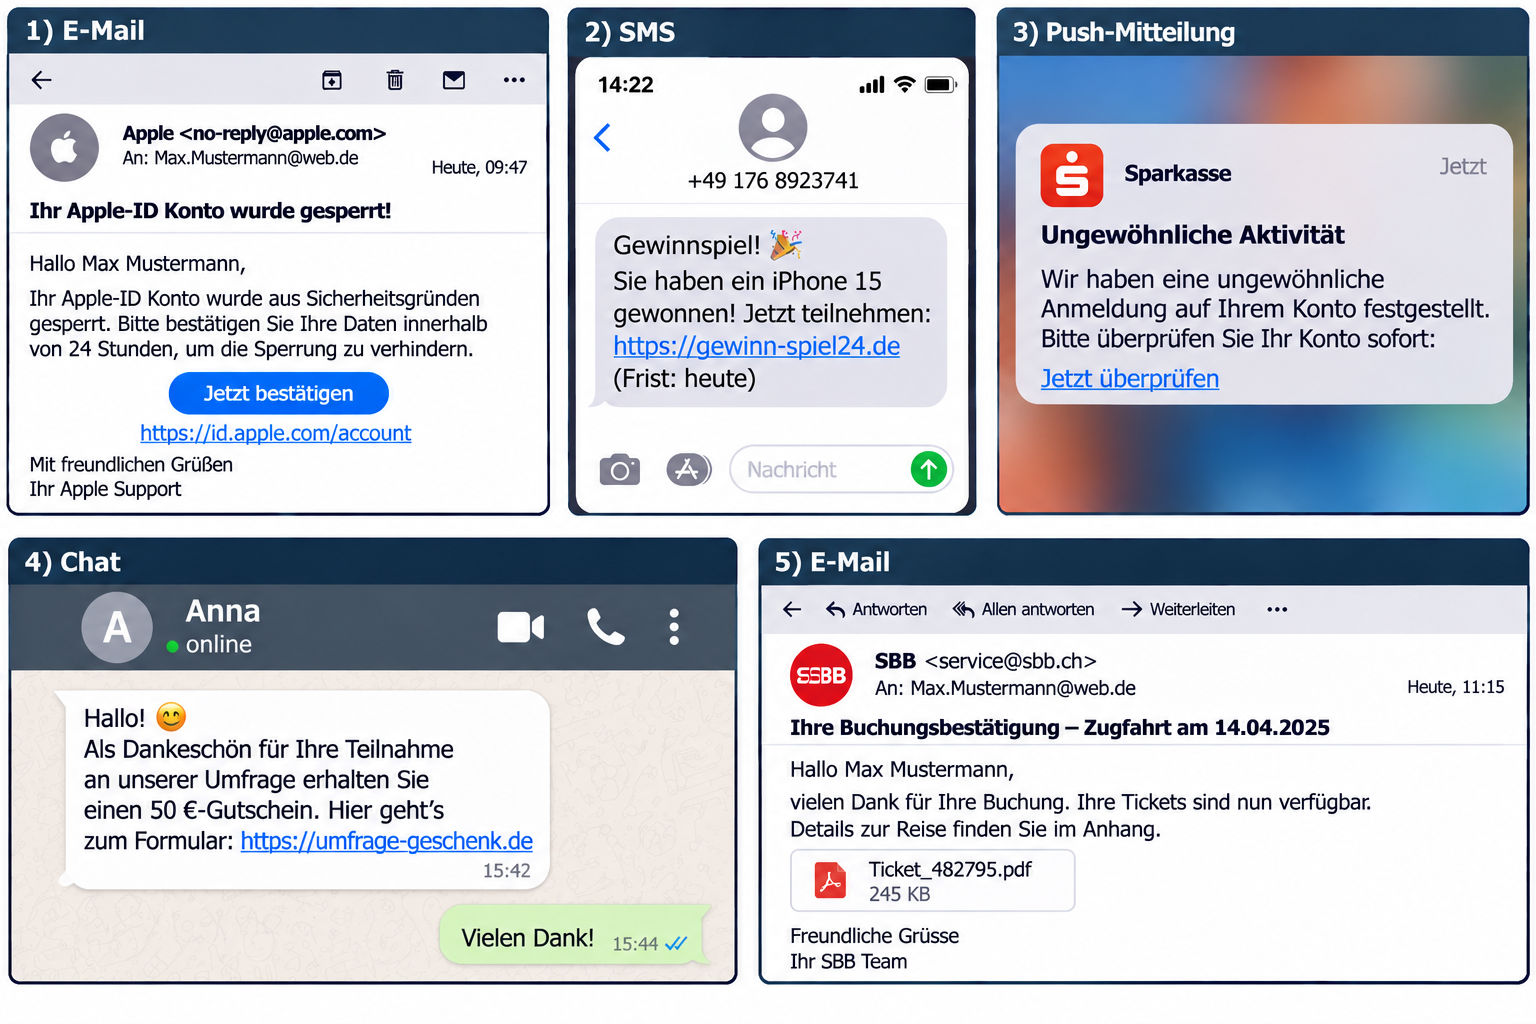
\includegraphics[width=0.9\textwidth]{Fünf digitale Nachrichten im Überblick.png}
    \caption[5 Nachrichten]{5 digitale Nachrichten im Überblick (erstellt mit DALL-E, 22.11.2026).}
    \label{fig:5_nachrichten}
\end{figure}
\end{taskbox}

\begin{solutionbox}[Musterlösung Aufgabe 9]
\begin{enumerate}[label=\alph*)]
    \item \textbf{Verdächtige und vertrauenswürdige Merkmale im Überblick:}
    \begin{enumerate}
        \item \textbf{E-Mail Apple (Legitim):}
        \begin{itemize}
            \item \textit{Absender:} \texttt{no-reply@apple.com}, offizielle Apple-Domain.
            \item \textit{Link:} \texttt{https://id.apple.com/account}, gehört zur Domain \texttt{apple.com}.
            \item \textit{Tonfall:} Aufforderung zur Kontobestätigung, wirkt zunächst dringend.
            \item \textit{Vertrauenswürdiges Merkmal:} Absender und angegebener Link passen zu Apple.
        \end{itemize}

        \item \textbf{SMS iPhone-Gewinnspiel (Phishing):}
        \begin{itemize}
            \item \textit{Absender:} Unbekannte Telefonnummer.
            \item \textit{Link:} \texttt{gewinn-spiel24.de}, keine offizielle Apple-Domain.
            \item \textit{Tonfall:} Verspricht einen kostenlosen iPhone-Gewinn.
            \item \textit{Verdächtiges Merkmal:} Zeitdruck durch die Aussage „Frist: heute“.
        \end{itemize}

        \item \textbf{Push-Mitteilung Sparkasse (Phishing):}
        \begin{itemize}
            \item \textit{Absender:} Angebliche Sparkasse.
            \item \textit{Link:} Die tatsächliche Zieladresse ist nicht sichtbar.
            \item \textit{Tonfall:} Erzeugt Angst durch eine angeblich ungewöhnliche Kontoaktivität.
            \item \textit{Verdächtiges Merkmal:} Aufforderung, das Konto sofort zu überprüfen.
        \end{itemize}

        \item \textbf{Chat Anna (Phishing):}
        \begin{itemize}
            \item \textit{Absender:} Anna, scheinbar eine bekannte Kontaktperson.
            \item \textit{Link:} \texttt{umfrage-geschenk.de}, keine erkennbare offizielle Unternehmensdomain.
            \item \textit{Tonfall:} Freundlich und verlockend durch einen 50-Euro-Gutschein.
            \item \textit{Verdächtiges Merkmal:} Ungewöhnliches Gutscheinangebot über einen externen Link.
        \end{itemize}

        \item \textbf{E-Mail SBB (Legitim):}
        \begin{itemize}
            \item \textit{Absender:} \texttt{service@sbb.ch}, offizielle SBB-Domain.
            \item \textit{Domain:} \texttt{sbb.ch}, offizielle Webseite der Schweizerischen Bundesbahnen.
            \item \textit{Tonfall:} Sachlich und informativ.
            \item \textit{Vertrauenswürdige Merkmale:} Konkrete Buchungsbestätigung und passender Reisebezug.
        \end{itemize}
    \end{enumerate}

    \item \textbf{Zusammenfassende Zuordnung:}
    \begin{itemize}
        \item \textbf{Legitime Nachrichten:} Beispiel 1 (E-Mail Apple) und Beispiel 5 (E-Mail SBB).
        \item \textbf{Phishing-Nachrichten:} Beispiel 2 (SMS iPhone-Gewinnspiel), Beispiel 3 (Push-Mitteilung Sparkasse) und Beispiel 4 (Chat Anna).
    \end{itemize}
\end{enumerate}
\end{solutionbox}

\begin{taskbox}[{Aufgabe 10: MFA und Live-Phishing durchschauen}]
\begin{enumerate}[label=\alph*)]
    \item Ein Mitschüler behauptet: \textit{Solange ich SMS-Codes oder eine Authenticator-App aktiviert habe, kann mir auf einer gefälschten Login-Seite nichts passieren.} Erklären Sie Schritt für Schritt, wie ein Angreifer diese Schutzmassnahme mithilfe von \textbf{Live-Phishing} trotzdem überwindet.
    \item Warum funktionieren \textbf{TOTP-Codes} und \textbf{Push-Mitteilungen} auf einer gefälschten Zwischenseite, während ein \textbf{Passkey} oder \textbf{FIDO2-Schlüssel} den Login blockiert?
\end{enumerate}
\end{taskbox}

\begin{solutionbox}[Musterlösung Aufgabe 10]
\begin{enumerate}[label=\alph*)]
    \item Beim Live-Phishing schaltet der Angreifer eine gefälschte Zwischenseite zwischen das Opfer und die echte Website. Gibt das Opfer dort Passwort und Einmalcode ein, leitet die Zwischenseite beides in Echtzeit an den echten Dienst weiter und fängt das anschliessend ausgestellte \textbf{Session-Cookie} ab. Damit ist der Angreifer direkt im Konto eingeloggt.
    \item TOTP-Codes hängen nur vom geheimen Schlüssel und der Uhrzeit ab (nicht von der Website), und Push-Bestätigungen löst der Angreifer durch seinen eigenen Anmeldeversuch selbst aus. Passkeys und FIDO2-Schlüssel sind hingegen kryptografisch an die \textbf{exakte Domain} des echten Dienstes gebunden und verweigern auf der gefälschten Seite den Dienst.
\end{enumerate}
\end{solutionbox}

\newpage
\subsubsection{Teil 3: Notfallplan \& Praxis-Transfer}
\begin{taskbox}[{Aufgabe 11: Notfallplan}]
Ein Freund schreibt Ihnen panisch: \textit{Ich habe gerade auf einen Link in einer angeblichen Paket-SMS geklickt und meine private E-Mail-Adresse sowie mein Passwort eingegeben, keine Bank-Angaben. Erst danach habe ich gemerkt, dass die Seite gefälscht war! Ich nutze dieses Passwort leider auch für andere private Dienste. Was soll ich jetzt tun?}

Lesen Sie auf Moodle (\textit{Auf einen Phishing-Link geklickt oder Daten eingegeben?}) den Text und erstellen Sie einen strukturierten Notfallplan, mit dem Ihr Freund den Schaden sofort begrenzt. Begründen Sie jeden Schritt kurz.
\end{taskbox}

\begin{solutionbox}[Musterlösung Aufgabe 11]
\begin{enumerate}
    \item \textbf{Passwörter sofort ändern \& MFA aktivieren:}
    \begin{itemize}
        \item \textit{Betroffenes Konto sichern:} Das Passwort des betroffenen Dienstes umgehend über die echte, manuell aufgerufene Website (nicht über den SMS-Link!) ändern, damit die Angreifer keinen Zugriff mehr haben.
        \item \textit{Weitere Konten \& E-Mail schützen:} Da das Passwort mehrfach genutzt wurde, müssen sofort alle anderen Dienste (insbesondere das E-Mail-Hauptkonto, da darüber per \textit{Passwort vergessen} andere Konten übernommen werden können) ein eigenes, starkes Passwort erhalten.
        \item \textit{\gls{mfa} einschalten:} Wo immer möglich, sofort eine Zwei-Faktor-Authentifizierung aktivieren.
    \end{itemize}

    \item \textbf{Beweise sichern \& Vorfall in der Schweiz melden:}
    \begin{itemize}
        \item \textit{Beweise aufbewahren:} Die Smishing-Nachricht nicht sofort löschen, \\ sondern Screenshots (inkl. Absendernummer und Link) erstellen.
        \item \textit{Melden:} Den Vorfall über das Meldeformular des Bundesamts für Cyber-Sicherheit (\textbf{BACS}, \texttt{report.ncsc.admin.ch}) bzw. \texttt{antiphishing.ch} melden (und bei finanziellem Schaden Strafanzeige bei der Polizei \mbox{erstatten}). 
    \end{itemize}
\end{enumerate}
\end{solutionbox}

\begin{taskbox}[{Aufgabe 12: Praxis-Check der eigenen Konten}]
Überprüfen Sie (ohne sensible Daten preiszugeben!) die Sicherheit Ihrer mindestens zwei wichtigsten persönlichen Online-Konten (z.\,B. privates E-Mail-Konto, Apple-ID, Google-Konto, Instagram, Snapchat).
\begin{enumerate}[label=\alph*)]
    \item Prüfen Sie in den Sicherheitseinstellungen der jeweiligen Dienste, ob \textbf{\gls{mfa}} aktiviert ist und welches Verfahren aktuell genutzt wird (SMS-Code, Authenticator-App, Push-Mitteilung oder Passkey).
    \item Bewerten Sie für jedes dieser Konten, ob die aktuelle Absicherung auch gegen \textbf{Live-Phishing} schützt, und notieren Sie eine konkrete Verbesserung, die Sie heute noch umsetzen können.
\end{enumerate}
\end{taskbox}

\begin{solutionbox}[Musterlösung Aufgabe 12]
\textit{(Individuelle Schülerlösung, Beispielhafte Auswertung:)}
\begin{itemize}
    \item \textbf{Konto 1 (Google-Konto/Apple-ID):} MFA ist aktiv über Push-Mitteilung. \textit{Bewertung:} Schützt gegen klassisches Phishing, aber nicht gegen Live-Phishing. \textit{Verbesserung:} Zusätzlich einen Passkey (FaceID/TouchID) einrichten.
    \item \textbf{Konto 2 (Instagram/Snapchat):} MFA ist noch deaktiviert (nur Passwort). \textit{Bewertung:} Sehr hohes Risiko einer Kontoübernahme. \textit{Verbesserung:} Sofort MFA per Authenticator-App aktivieren (SMS vermeiden, da \mbox{unsicherer}).
    \item \textbf{Konto 3 (Microsoft 365):} MFA über Microsoft Authenticator aktiv. \textit{Bewertung:} Guter Basisschutz; bei Anmeldeanfragen stets genau prüfen, ob man den Login selbst ausgelöst hat, und auf die URL achten.
\end{itemize}
\end{solutionbox}

\newpage
% --- LITERATURVERZEICHNIS & AKRONYME (AUF EINER GEMEINSAMEN SEITE) ---
\printbibliography[heading=bibintoc, title={Literaturverzeichnis}]

\vspace{1.5cm}
\printglossary[type=\acronymtype, title=Akronyme]

\newpage
% --- GLOSSAR (AUF EINER SEPARATEN SEITE) ---
\printglossary[title=Glossar]

\end{document}
